\section{Program-of-Thought and Code-Assisted Reasoning}

\begin{frame}{}
    \LARGE Advanced Reasoning: \textbf{Code-Assisted Reasoning}

    \vspace{1em}
    \normalsize What changes when part of the reasoning is executed by an interpreter?
\end{frame}

\begin{frame}{Program of Thoughts: Separate Reasoning from Computation}
    \begin{columns}[T,onlytextwidth]
        \column{0.55\textwidth}
        \begin{itemize}\itemsep0.45em
            \item \textbf{Program of Thoughts (PoT)} appeared alongside PAL in 2022. Zero-shot, it beats CoT on every benchmark tested (right). It is within 0.4 points of PAL on GSM8K.
            \item \textbf{What lasts is the ablation.} GSM8K: full method 71.6. Variables renamed to a, b, c: 60.2. One direct equation: 45.8. Multi-step programs and \emph{semantic binding} do the work.
            \item \textbf{And the error analysis.} Of 198 failures on one benchmark, 47\% are \emph{value grounding}. Code does not fix that.
        \end{itemize}
        \column{0.42\textwidth}
        \centering
        \small
        \textbf{Zero-shot accuracy (\%)}

        \vspace{0.3em}
        \begin{adjustbox}{max width=\linewidth}\begin{tabular}{lcc}
            \toprule
            \textbf{Benchmark} & \textbf{CoT} & \textbf{PoT} \\
            \midrule
            GSM8K & 40.5 & 57.0 \\
            AQuA & 31.9 & 43.9 \\
            SVAMP & 63.7 & 70.8 \\
            TabMWP & 53.5 & 66.5 \\
            MultiArith & 79.3 & 92.2 \\
            \rowcolor{KAUSTcyan!12} Average & 53.7 & 66.1 \\
            \bottomrule
        \end{tabular}\end{adjustbox}
    \end{columns}
    \vspace{0.2em}
    \src{Chen, Ma, Wang and Cohen, ``Program of Thoughts Prompting,'' TMLR 2023, \href{https://arxiv.org/abs/2211.12588}{arXiv:2211.12588}, Tables 3, 5 and 6. Gao et al., ``PAL: Program-aided Language Models,'' \href{https://arxiv.org/abs/2211.10435}{arXiv:2211.10435}.}
\end{frame}

\begin{frame}{Chain of Code: When a Line Cannot Run, Simulate It}
    \centering
    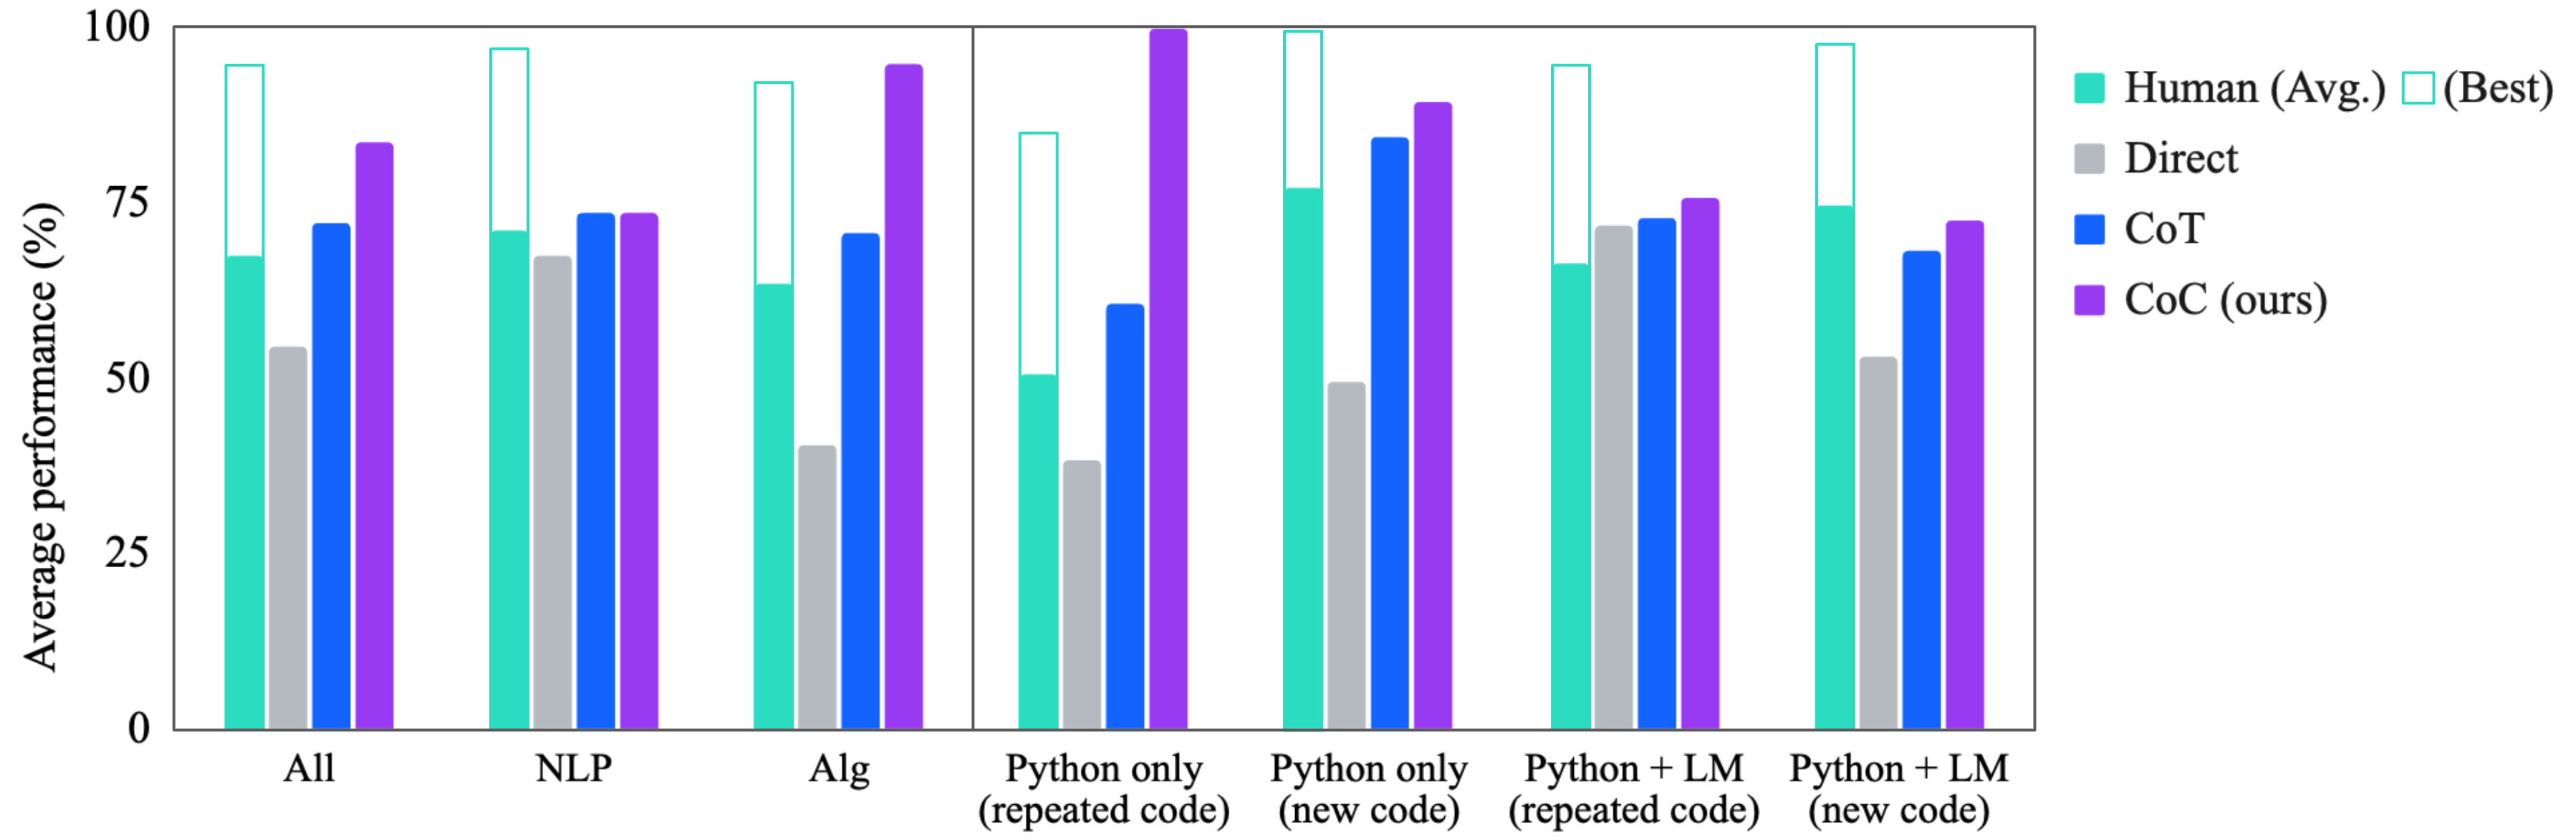
\includegraphics[width=0.84\linewidth,height=0.38\textheight,keepaspectratio]{images/advanced-reasoning/coc_by_task_type.png}
    \begin{itemize}\itemsep0.3em
        \item \textbf{Problem:} many reasoning steps are semantic. No library implements \texttt{is\_sarcastic(s)}.
        \item \textbf{Idea:} write code that mixes real code and pseudocode. Run it line by line. When a line fails, the language model \emph{simulates} its effect on the program state.
        \item BIG-Bench Hard: \textbf{84\%}, against 72\% for CoT and 68\% for the average human rater.
        \item The ablation that matters: \textbf{Python alone gives 48\%}. The language model alone tracking state gives 63\%.
    \end{itemize}
    \src{Li et al., ``Chain of Code,'' ICML 2024, \href{https://arxiv.org/abs/2312.04474}{arXiv:2312.04474}, Figure 4 and Tables 1 and 2. Model: text-davinci-003.}
\end{frame}

\begin{frame}{From Prompted Programs to Trained Tool Use}
    \begin{columns}[T,onlytextwidth]
        \column{0.42\textwidth}
        \centering
        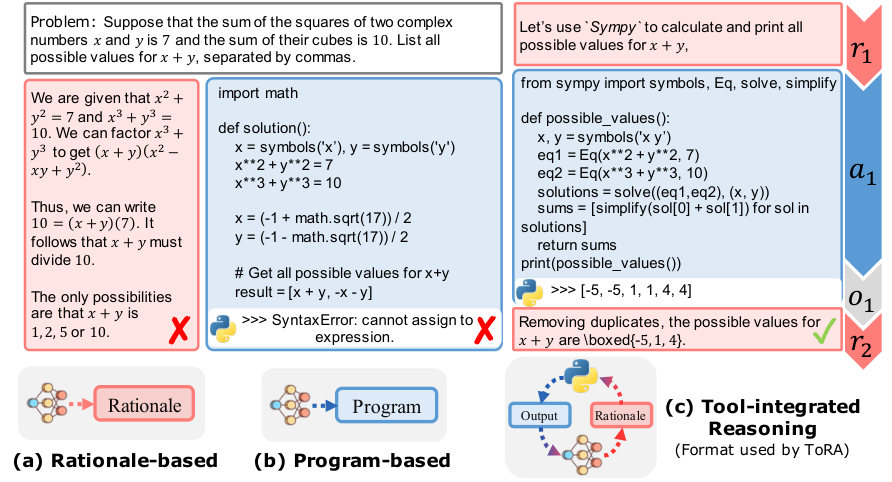
\includegraphics[width=\linewidth,height=0.5\textheight,keepaspectratio]{images/advanced-reasoning/tora_pipeline.png}

        \vspace{0.2em}
        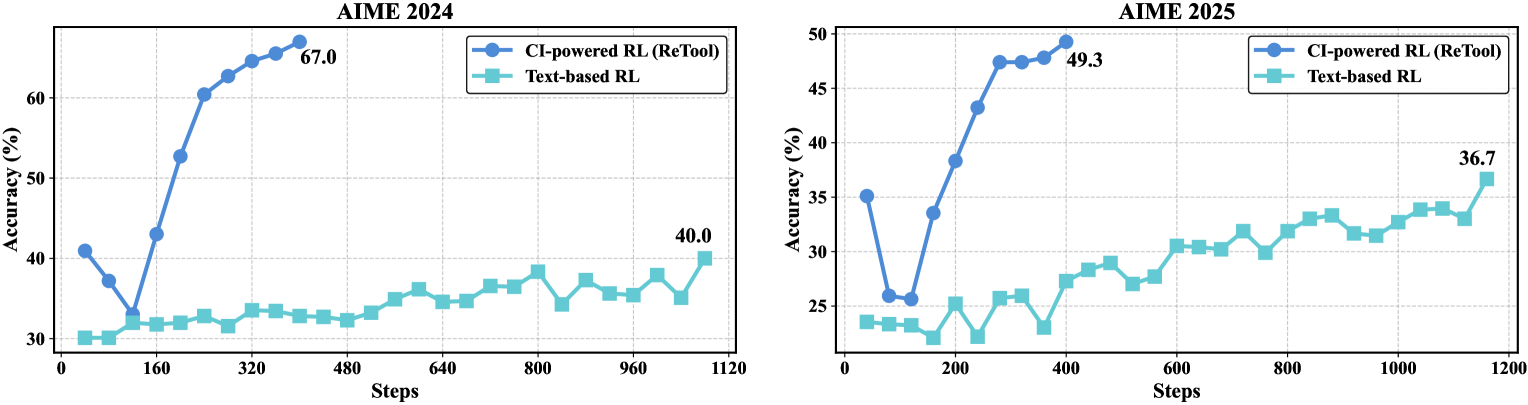
\includegraphics[width=\linewidth,height=0.2\textheight,keepaspectratio]{images/advanced-reasoning/retool_fig1_aime_training.png}
        \column{0.56\textwidth}
        \begin{itemize}\itemsep0.4em
            \item \textbf{ToRA (supervised).} Interleave rationale $r_i$, program $a_i$ and interpreter output $o_i$:
            $\tau = r_1 a_1 o_1 \dots r_{n-1} a_{n-1} o_{n-1} r_n$.
            It beats program-only by 6.7 points.
            \item \textbf{ReTool (RL).} Run a real sandbox \emph{inside} the rollouts. Two details recur in later systems:
            \begin{itemize}\itemsep0.1em
                \item interpreter output is masked out of the loss
                \item the reward is the outcome only: $+1$ or $-1$
            \end{itemize}
            \item AIME 2024 with a 32B model: \textbf{67.0\% in 400 steps}. Text-only RL: 40.0\% in 1,080 steps. Responses get about 40\% shorter.
            \item The model learns \emph{when} to call code, and to repair it from error messages.
        \end{itemize}
    \end{columns}
    \vspace{0.1em}
    \src{Gou et al., ``ToRA,'' ICLR 2024, \href{https://arxiv.org/abs/2309.17452}{arXiv:2309.17452}. Feng et al. (ByteDance Seed), ``ReTool,'' \href{https://arxiv.org/abs/2504.11536}{arXiv:2504.11536}, Figure 1 and Table 1.}
\end{frame}

\begin{frame}{When Code Hurts}
    \begin{itemize}\itemsep0.5em
        \item A study of 7 methods, 14 tasks and 6 models asks: is code always the better choice?
        \item \textbf{Text beats code on planning tasks.} Correct code would have to combine constraint checking, optimisation and simulation.
        \item \textbf{Inverse scaling.} On Game of 24, GPT-3.5 and GPT-4o-mini reach 100\% because they always write code. \alert{GPT-4o is overconfident in text and skips the code} on medium questions.
        \item \textbf{With feedback over several turns,} code methods keep improving. Text-only self-reflection degrades.
    \end{itemize}
    \vspace{0.2em}
    \takeaway{Code for \emph{execution}: exact computation, enumeration, checking. Language for \emph{grounding and planning}. The best systems interleave both.}
    \src{Chen et al., ``Steering Large Language Models between Code Execution and Textual Reasoning,'' ICLR 2025, \href{https://arxiv.org/abs/2410.03524}{arXiv:2410.03524}. Li et al., \href{https://arxiv.org/abs/2312.04474}{arXiv:2312.04474}. Chen et al., \href{https://arxiv.org/abs/2211.12588}{arXiv:2211.12588}.}
\end{frame}

\begin{frame}{Code-Assisted Reasoning: What to Remember}
    \begin{itemize}\itemsep0.6em
        \item Code separates \textbf{what to compute} from \textbf{computing it}. The interpreter is an exact executor.
        \item The gain comes from \textbf{multi-step programs with meaningful names}, and from interleaving code with language.
        \item The lineage: one program run once, then a simulated interpreter, then supervised tool use, then tool use \textbf{learned by outcome RL} and built into o3 and o4-mini.
        \item Code does not fix \textbf{grounding errors}, and it can make planning worse.
    \end{itemize}
    \vspace{0.3em}
    \begin{block}{A common misconception}
        ``A code interpreter always helps with mathematics.'' It helps with computation. It does not check that the reasoning around the computation is sound.
    \end{block}
    \vspace{0.3em}
    \takeaway{\textbf{Next.} Execution checks arithmetic. What would it take to check a whole \emph{argument}? That is the job of mathematical verification.}
\end{frame}
